\documentclass[twoside,openright,a4paper,11pt,french]{article}
\usepackage[utf8]{inputenc}
\usepackage[french]{babel}
\usepackage[T1]{fontenc}
\usepackage{emptypage}

% Utilisation d'url
\usepackage{url}
\urlstyle{sf}

% Utilisation d'images, stockées dans le répertoire ./pics/
\usepackage{graphicx}
\graphicspath{pics/}

% Définition des marges
\usepackage{geometry}
\geometry{
  left=25mm,
  right=25mm,
  top=25mm,
  bottom=25mm,
  foot=15mm
}

\begin{document}

\pagestyle{plain}

% La page de garde
\thispagestyle{empty}

\begin{center}
       \noindent
       \includegraphics[height=2.5cm]{./pics/uds.eps}       
       
       \vfill\vfill

    {\large \textsc{Licence 3 de Sciences, mention Informatique}}

    \bigskip\bigskip

    {\large \textsc{Réseaux et Protocoles}}

    \vfill\vfill

% Titre du document
    {\huge \sc
      \begin{center}
		Rapport d'étude du protocole IPv4
      \end{center}}

    \vfill\vfill

    {\large Présenté par}

\medskip

% Identité des auteurs
    {\large Luigi  \textsc{Coniglio}}\\
    {\large Victor \textsc{Constans}}\\
    {\large Daniel \textsc{Wilhelm}}\\
    {\large Moussa \textsc{Idrissa-Mossi}}

\bigskip

\end{center}



% La table des matières
\parskip=0pt
\tableofcontents

\section{Introduction}
\label{sec:intro}

Dans les réseaux locaux, les machines peuvent communiquer directement les unes
avec les autres par le biais d'un lien physique.\footnote{Ce lien peut directe
de machine à machine, ou indirecte: passant par d'autre équipement (switch,
hub,...).} En revanche, établir un lien entre des machines sur des réseaux
différents n'est pas aussi facile, cela pose en effet deux problèmes majeurs:
\begin{itemize}
\item Deux réseaux différents n'utilisent pas forcement la même technologie
pour transmettre des données au niveau protocolaire ou du lien physqiue.
\item Comme les machines ne sont pas physiquement sur le même réseau, il faut
un système d'adressage afin qu'une machine puisse joindre une autre machine
située dans un réseau différent, peu importe sa localisation.
\end{itemize}
Dans le cadre d'une communication, il est souvent pratique de diviser les
fonctionnalités nécessaire à l'échange d'information.  Pour cette raison il est
utile de définir un modèle théorique pour séparer les différentes tâches.
Aujourd'hui le standard en terme de modèle de communication est le modèle OSI
({\it Open Systems Interconnection}), qui divise en 7 couches les
fonctionnalités en question.

\bigskip
Le problème relatif à l'interconnection des réseaux (vu plus haut) est traité
par la couche 3 (nommé couche réseau) du modèle OSI.
Cette couche peux être fonctionnellement mise en oeuvre par le protocole IPv4.
C'est actuellement le protocole réseau (relative à la couche 3 du modèle OSI)
le plus utilisé et qui à permit le déployement massive d'Internet dans le
monde.\\
Dans la suite de ce rapport, nous allons étudier le fonctionnement d'IPv4, les
possibilités qu'il offre et l'écosystème de protocoles qui gravitent autour
d'IPv4 et qui sont nécessaires à son bon fonctionnement.  Nous allons commencer
par explorer le contexte de création de ce protocole et comprendre les
motivations qui ont pousser le concevoir.





% ------------------------------------------------

La technique de classe d'adressage IP ( classful network ) est une méthode utilisée de 1981 à 1993 pour allouer des adresses IPV4. Il a été défini en 1981 qu'une adresse IP est divisée en deux parties : une partie qui sert à identifier le réseau et une partie qui sert à identifier une interface sur ce réseau.
Dans cette méthode une adresse IP est divisée en 5 plages d'adresses IP et sont appelées classes. Ils sont organisés comme dans le tableau ci-dessous  :

\includegraphics{./pics/tableau.eps}


Chaque classe a un certain nombre d'octets servant à identifier le réseau. Une adresse IP de classe A à un identificateur de réseau sur 1 seul octet. Une adresse IP de classe B sur 2 octet et une de classe C sur 3 octets. Les adresses IP de classe D et E correspondent à des adresses IP particulières.
Les réseaux des différentes classes utilisent un certain nombre d'octets pour identifier le réseau. Ils ont donc un nombre différent d'octets restants qu'ils peuvent donner à des interfaces. 
Pour déterminer à quelle classe appartient une adresse IP il suffit de regarder les premiers bits de l'adresse.
Afin d'avoir un niveau supplémentaire, grâce auquel on gagne en flexibilité et en efficacité dans l'attribution d'adresse à l'intérieur d'une classe, on a introduit le concept de sous-réseau. Celui-ci introduit un nouveau numéro entre le numéro de réseau et le numéro d'hôte. Grâce aux sous-réseaux on peut par exemple diviser une adresse de classe B en 256 sous-réseaux pouvant chacun avoir 256 interfaces connectées.
On utilise un masque de sous-réseau pour obtenir la partie réseau de l'adresse IP. Le masque de sous-réseau est obtenu en mettant tous les bits de la partie réseau à 1 et tous les bits de la partie interface à 0. Lorsque deux adresses IP appartiennent au même sous-réseau, elles ont en commun les bits identifiants ce sous-réseau. Pour déterminer si 2 interfaces appartiennent au même sous-réseau, on les compare donc d'abord au masque de sous-réseau puis on les compare entre elles.
Cependant, ce système d'adressage a un grand inconvénient. En effet, il n'existe que 4 classes différentes et donc 4 types de réseaux de taille différentes. Cela conduit souvent à de grand gaspillage d'adresse. Par exemple, lorsqu'une entreprise souhaite une adresse IP. Si celle-ci possède 2000 interfaces, une adresse de classe C (2⁸ hôtes possibles) ne sera pas suffisante. Une adresse de classe B sera par contre largement trop grande (2¹⁶ hôtes possibles). C'est à cause de ce problème de gaspillage et du manque d'adresses IP que l'on est passé au   Classless InterDomain Routing (CIDR).

% ------------------------------------------------


\section{Concepts et utilisation}

Des données transmissent en utilisant le protocole IPv4 sont encapsulées dans un message que
l'on appelle un paquet IPv4. Ces paquets sont consitué d'un entête suivis des données à transmettre.

% Mossi
\subsection{Adresse IPv4}

L'entête contient des informations essentielles pour la transmission d'un paquet, notamment les
adresses source et destination.

Une adresse IP sert à identifier une machine (et plus précisement une des interfaces de cette machine)
dans un réseau particulié.
Comme nous le verrons plus tard cet identifiant unique permet de désigner à la fois un
réseau et une machine précise au sein de ce réseau.
Une adresse est codé sur 32 bits ce qui permet de coder 2\^32 soit 4294967296 adresses différentes.
Par convention on peut représenter une adresse IPv4 comme une suite de 4 nombres décimaux séparés par des points,
chacun traduisant un octet. Cette représentation a contribuée à simplifier l'utilisation et la manipulation
des adresses.
Comme chaque nombre représente un octet, les valeurs de celui-ci sont comprises entre 0 et 255.

\vspace{1cm}
Exemple: adresse à valeur décimale: 212.217.0.1 => correspond sous sa forme
binaire à: 11010100.11011001.00000000.00000001
\vspace{1cm}

\subsubsection{Notion de NET ID et HOST ID}
Une adresse IPv4, en tant qu'inditifiant d'une machine dans un réseau, contient deux informations:
une première partie qui identifie le réseau appellé NET ID (les bits de poids fort), une seconde qui identifie l’hôte appeler host-ID (les bits de poids faible).
Les machines qui se trouvent donc sur le même réseau partage le même NET ID pour leur adresse.

La longueur de ces deux parties est variable: la taille du HOST ID dépend de la taille du NET ID. Pour représenter la longueur de ces différentes parties on a introduit la notion de masque

\subsubsection{Masque de réseau}

Le masque sert à représenter la scission entre le NET ID et le HOST ID.
Il est codé sur 32 bits et adopte la même représentation qu'une adresse IP, à savoir
4 nombres décimaux séparé par des points.
La position des bits à 1 dans le masque corresponde à la position des bits définissant le NET ID dans l'adresse IP.
Pour obtenir les bits du NET ID il suffit de faire un ET logique entre l'adresse et son masque. Tous les autres bits (donc les bits à 0)
feront donc partie du HOST ID.
Les bits à 1 sont contiguës et commencent au bit de poids fort: le nombre de bit à 1 dans le masque, donne
le nombre de bit faisant partie du NET ID en partant du bit de poids fort dans l'adresse.

En conséquence plus le nombre de bit à 1 dans le masque est grand, plus le NET ID sera grand, et plus le HOST ID sera petit, car il restera moins de bit pour définir le HOST ID (la somme des deux devant évidemment faire 32 bits).

\begin{center}
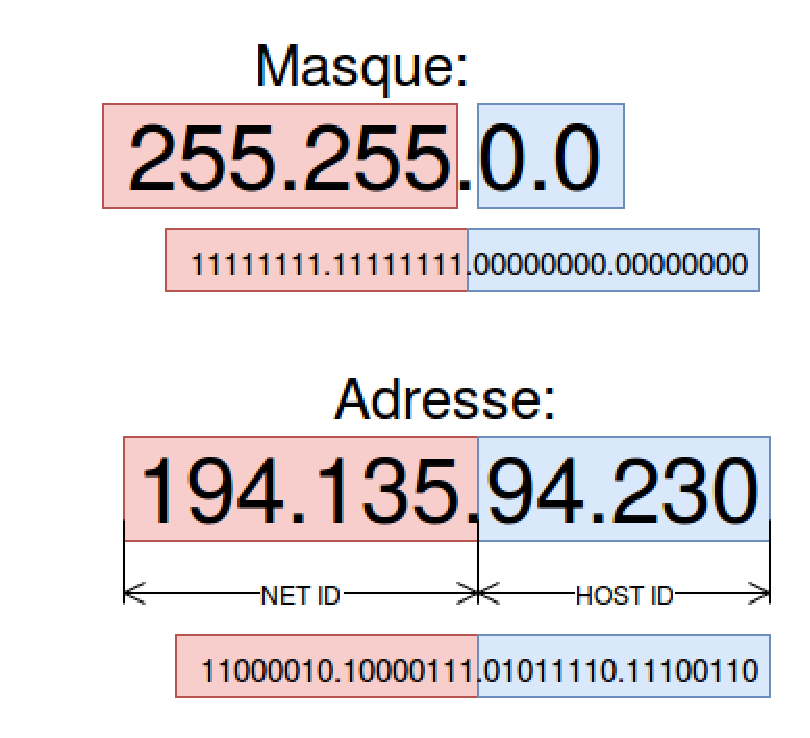
\includegraphics[width=7cm]{./pics/maskipv4.eps}
\end{center}

//TODO exemple
//TODO exemple invalide

\subsubsection{Classes d'adresse IP}
Historiquement les classes d'adresse IP correspondaient à une plages d'adresses avec un masque figer pour une classe donnée.
Ce système permettait de déduire le masque en fonction
de l'adresse IP étant donné que chaque classe avait son masque défini de manière standard.
Il fut décrit dans le RFC 791\cite{url-RFC-791}.

//TODO tableau classe

A partir de ce tableau nous pouvons voir qu'il suffit de regarder les 4 bits de
poids fort pour déduire à quelle classe appartient une adresse.  Par exemple si
une machine à pour adresse 152.123.87.45 on sait en regardant les 4 premiers
bits que cette adresse fait partie de la classe B (car l'adresse commence par
10). De là, la machine n'a pas besoin de masque en plus car elle sait que le
masque correspondant un adresse de classe B est 255.255.0.0 .

Ce système permet donc d'adresser de nombreux réseaux avec un nombre de machine
variable en fonction de la classe, et tout cela sans avoir besoin de
communiquer ou de paramétrer un masque; celui-ci étant normalisé pour chaque
classe.  Cependant il a un gros inconvénient, étant donné que les masques sont
figé, un réseau peux ne peux pas utiliser une partie plus ou moins importante
de ses adresses. Par exemple si un réseau contient 500 machines, il ne peux pas
utiliser d'adresse de classe A étant donné que celle-ci ne permettent d'avoir
que des réseaux de 254 machines maximum. Il va donc falloir utiliser des
adresses de classe B minimum, car elles permettent d'adresser 65534 machines au
sein d'un réseau. Nous pouvons donc utiliser 500 adresses sur les 65534
disponible, mais le reste sera "perdu".  Ce système était simpliste mais
n'était pas utilisable sur le long terme car il "gache" des adresses en
n'utilisant pas tout son espace d'adressage.


\subsubsection{CIDR}

Aujourd'hui le système le plus utilisé est CIDR (Classless Inter-Domain
Routing) remplace le système de classe d'adresse. CIDR permet de créer des
masque beaucoup plus fin, étant donné qu'on n'est plus limité à des masque de
réseau fixe, on peut ajuster le masque pour avoir le nombre de machine
adressable dans un réseau le plus proche possible du nombre de machine que l'on
souhaite adressé.  Cela permet de limiter les pertes en adresse inutilisé, si
la plage est correctement découpée.  On peut donc créer des masques à la
séparation entre le NET ID et le HOST ID se trouve n'importe où, même en plein
milieu des octets (ce qui était impossible avec les classes d'adresse), ce qui
apporte une plus grande fléxibilité.  Cela permet aussi de créer une hiérarchie
dans une plage d'adresse réseau qui serait découper en plusieurs réseaux
"fils", et cela permet notamment, avec cette hierarchie, de réduire la table de
routage des routeur.  De là est né une nouvelle notation des masques: on écrit
le nombre de bit à 1 dans le masque à la suite de l'adresse IP et séparé par un
slash.







\subsubsection{Types d'adresses}
La variété des exigences en matière de réseaux a donnée lieu à une
classification progressive des adresses selon des rôles bien precis. En effet,
pas toutes les adresses IPv4 ont la même signification: à certaines adresses
(ou plages d'adresses) ont été attribué par convention des fonctions ou
caracteristiques particulières.  Dans la suite de cette partie on analysera les
adresses IP sous trois aspects differants: on classifiera d'abord les adresses selon
le type de diffusion qu'elles permettant de effectuer, puis on introduira le
concept d'adresse publique et adresse prive, enfin on parlera des fonctions
speciales qui ont ete assigne a certaines adresses.


\paragraph{Types de diffusion}
Dans le cadre des trasmission en plus de communiquer avec une seule machine, on
a par fois la necessite que un message soit recu par un groupe de machines ou
meme la totalite d'une reseau.



%TODO portee d'un adresse: broadcast, multicast, anycast unicast%

\paragraph{Adresses publiques et adresses prive}

%Note: private --> 10.0.0.0/8, 172.16.0.0/12 192.168.0.0/16

\paragraph{Adresses speciales}
L'usage spéciale d'une adresse IP découlait de l'émergence
%TODO (apparition??) 
d'un nouveau besoin dans le domaine des réseaux; c'est pour
ça que jusqu'à 2002, l'attribution des rôles spéciaux des adresses
IPv4 était présentés dans divers document, qui présentaient, et répondaient à chaque fois à une
problématique bien particulière. Le RFC3330 est un des premiers documents à
rassembler les classification des adresses IPv4 selon leur rôles et significations.

%TODO lien%


\begin{description}
\item[0.0.0.0/8]
Cette plage d'adresses indique la machine courante dans le réseau courant.
Les adresses dans cette plage sont notamment utilisées dans certains protocoles de
configuration comme adresse source, lorsqu'une machine n'a pas encore d'adresse effective.
%RFC 1122 %

\item[127.0.0.0/8]
Une adresse appartenant a ce bloc est denommées adresse de {\it loopback}.  Un
paquet envoyé vers une telle adresse retourne directement chez l'expéditeur, sans sortir
du contexte de la machine émettrice. Parmi les adresses de cette plage,
127.0.0.1 est celle utilisée le plus fréquemment\footnote{Comme l'indique
le RFC 1122, certaines implémentations de l'adresse de {\it loopback} se
limitent à utiliser le bloc 127.0.0.1/32, ce qui se traduit par l'unique utilisation de
l'adresse 127.0.0.1 }: dans plusieurs contextes cet adresses est réferencée par
l'alias "{\it localhost}".\footnote{La correspondance entre le nom {\it localhost} et
l'adresse 127.0.0.1 est généralement mise en place par le système d'exploitation.
Dans les systèmes de type UNIX une entrée reliant ces deux entitées est généralement
présente dans le fichier "/etc/hosts".}
Une adresse de {\it loopback} n'a pas de sens en dehors
d'un host, et c'est pour cela qu'elle ne devrait apparaître à aucun moment dans le réseau.

%RFC 1122 %

\item[169.254.0.0/16]
Cet plage d'adresses a été désignée comme contenant les adresses qu'on appelle
de {\it lien local}.  Les adresses dit de {\it lien local} sont utilisée lorsque
une machine n'a aucun moyen d'obtenir une adresse IP (par example par le biais
d'un serveur DHCP ou simplement avec une configuration manuelle).  L'obtention
d'une adresse de {\it lien local} est faite de façon automatique à travers un
processus d'autoconfiguration souvent appellé par l'acronyme APIPA ({\it
Automatic Private Internet Protocol Addressing}) ou par le nom IPv4LL.  Le
fonctionnement du processus APIPA (decrit dans le RFC 3927) est assez complexe
 et entraîne l'utilisation de certaines fonctionnalitées du
protocole ARP (qu'on traitera plus en detail dans la section %TODO \ref{sec:suiteproc} % )
. Son focntionnement peut être synthétisé dans ses grandes lignes par la démarche suivante:

\begin{description}
\item[Selection de l'adresse]
La machine choisit aléatoirement
    \footnote{Il est conseillé d'utiliser l'adresse MAC de l'interface en question
    pour générer l'adresse de {\it lien local} pour qu'il y ait une plus forte chance
    qu'elle soit unique dans le reseau.} 
une adresse appartenant à la plage 169.254.0.0/16

\item[Sondage sur l'adresse]
Une fois qu'on a selectionné une adresse, il faut s'assurer que la même adresse ne soit
pas deja utilisée par d'autres machines sur le réseau. Dans ce but la machine
pose la question à toutes les autres machines du réseau au moyen d'un ou plusieurs messages
en brodcast, et attend une réponse pendant un certain intervalle de temps\footnote{
Des précautions sont prises pour éviter les conflits générés par plusieurs
machines qui effectuent simultanément cette action pour le même adresse,
notamment: des intervalles de temps aléatoires entre l'envoie des messages, la mise
en place d'une écoute active des autres messages pendant le temps de l'enquete.}
Le manque de réponse indique que l'adresse est bien unique. Si l'adresse n'est
pas unique il faut en choisir une autre.

\item[Annonciation de l'adresse]
A ce point la machine peut communiquer aux autres machines l'adresse qu'elle
vient de réserver.

\end{description}



Ce processus est basé sur le concept de {\it Zeroconf}: il permet la mise en
place d'un reseau IPv4 sans aucune configuration. Ce type de système,
C'est aussi grâce a ce genre de systèmes, qu'on 
pourrait synthétiser par la devise %TODO slogan??  
"plug and play", que le concept de Networking (et avec lui Internet) a pu se
diffuser assez rapidement: grâce à APIPA un réseau IPv4 peut être facilement
mis en place sans le besoin d'aucune connaissance technique.\\

La plage d'adresses 169.254.0.0/16, désigne une plage d'adresse privée: les
adresses de type {\it lien local} ne sont donc pas atteignables en dehors de
leur réseau de definition. 
Cette plage d'adresses pose par contre des limites par rapport aux autres
plages d'adresses privée car, à la différence des autres, elle ne peut pas être
divisée en sous réseaux\footnote{Ce qui est assez logique si on considère que
le processus d'obtention d'une adresse de {\it lien local} (APIPA) utilise
les liens "physiques" entre les machines pour communiquer, et il ne peut
 considérer aucune notion de sous-reseau.}
: en effet un paquet destiné à une adresse de {\it lien local} ne doit pas être
retrasmise par un hôte intermédiaire.\footnote{Dans le paquet destiné
a une adresse de {\it lien local} le champ TTL est usuellement mis a 1
pour empêcher des forwarding.}

\item[192.88.99.0/24]
Les adresses appartenant à ce bloc désignent des routeurs 
fournissants un service de type {\it 6to4}. Ce type de service
permet de relier des réseaux IPv4 avec des réseaux IPv6.
Les adresses dans cette plage sont traitées comme étant des adresses
de type {\it anycast}.


\end{description}




------------------------------------------
Alors on vient de voir que les adresses IP privées sont utilisable uniquement
sur des réseaux locaux, tandis qu’il y a des adresses IP qui ne sont utilisées
uniquement que sur internet donc nous pouvons en déduir que c’est les adresses
IP publiques non utilisable dans un réseau local. Les routeurs (par exemple:
votre box) ont une adresse IP publique du côté d’internet, ce qui permet de
rendre votre box visible sur internet (elle répondra certainement au ping). De
plus, au moment de vos connexion sur un site web vous utilisez l’adresse
publique du serveur web. De ce fait une adresse IP publique est unique dans le
monde, ce qui n’est pas le cas dans le systèmes d’adressage des adresses IP
privées qui doivent être unique seulement dans un même réseau local mais pas au
niveau planétaire étant donné que ces adresses ne peuvent pas être routées sur
internet. Une adresse IP publique est soit acheté ou fournie par la FAI.  Les
IP publiques représentent toutes les adresses IP des classes A, B et C qui ne
font pas partie de la plage d’adresses privées de ces classes ou des exceptions
de la classe A (voir Adresse non utilisé ci-dessus).


\subsubsection{Les classes d’adresses}
Au début de la création de IPV4, maintes groupes d’adresses ont été définis
pour faciliter le routage (ou cheminement) des paquets. Structurée en 5 classes
(A,B,C,D,E) selon la valeur du première octet.

%TODO images classes %
%TODO tableau recapitulatif %

De ce fait on remarque une distribution de l’espace d’adressage selon laquelle
la classe A possède 50\% l’espace et soit 25\% pour la classe B, 12,5\% classe
C et 6,25\% pour D \& E. on peut en-déduire une mauvaise répartition de cette
espace d’adressage. 

%--------------------------------------
Les classes A, B et C ont chacune une correspondance de plage
d’adresses IP privées à l’intérieur de la plage globale qui a été définie par
la RFC 1918. Mais l’utilisation  de celui-ci pour inter-connecter des réseau
géante (entreprise) avec des espaces adressage qui se chevauche peut causer des
problèmes. Une adresse IP privées est librement paramétrée par l’administrateur
du réseau local.
Les adresses privées de la classe A: 10.0.0.0 à 10.255.255.255\\
Les adresses privées de la classe B: 172.16.0.0 à 172.31.255.255\\
Les adresses privées de la classe C: 192.168.1.0 à 192.168.255.255\\


\textbf{Remarque:}
De ce fait on distingue deux adresses particulières parmi tout ceux possible,
qui ne doivent jamais être attribué à des machines:

     les bits Host-ID sont à 0 : adresse attribue qu’à un réseau.
Exemple: 192.168.10.0 / 255.255.255.0 = 192.168.10.00000000

    les bits Host-ID sont à 1 : c’est un adresse de  diffusion (broadcast),
Exemple: 172.27.255.255 / 255.255.0.0 = 172.27.1111111.11111111

Donc nous pouvons en déduire que parmi tout les adresses assignable, ces
derniers sont des adresses interdites.



\subsubsection{Adresses non utilisées}
il existe des adresses non utilisable comme adresse IP pour une machine:\\
les adresses réseaux: qui correspond aux adresses qui ont tous les bits de
leur partie hostid à zéro(0);\\
les adresses de diffusion (broadcast): qui correspond aux adresses qui ont
tous les bits de leur partie hostid à un(1)\\
0.0.0.0: utilise par différentes services (table de routage, DHCP) et possède
souvent une signification particulières. \\
127.X.X.X: désigne l’ordinateur lui-même ou dite adresse de bouclage
(lookback), 127.0.0.1 pour le localhost\\
> à 223.255.255.255: pour le multicast et la recherche.\\




% Luigi Coniglio 
\subsection{En-tete IPv4}
Un packet IPv4 est precede` par un en-tete ayant une longeur minimale de 20 octets 
(dans les cas aucune option supplementaire a ete specifie`).
La figure suivante montre le contenu de l'en-tete d'un packet IPv4.


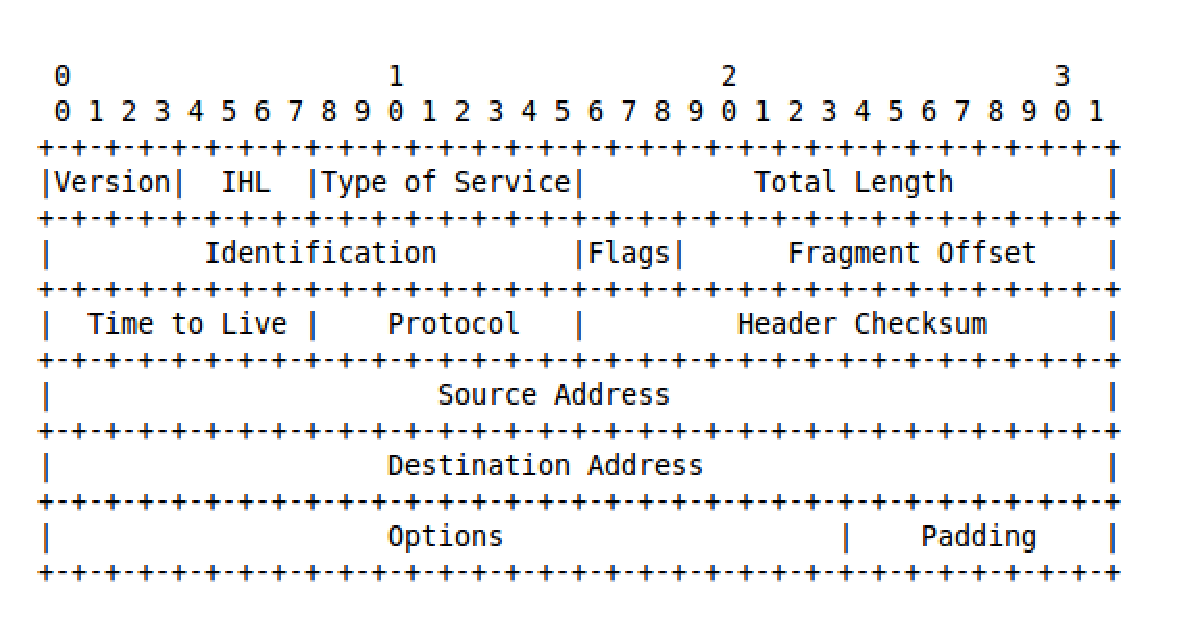
\includegraphics[width=15cm]{./pics/IPv4header.eps}


Comme on peut voir dans la figure ci dessus, un en-tete IPv4 est compose` par
13 champs, plus le padding. En realite nous verrons plus loin que cet en-tete
peut, quand il est necessaire, contenir un champ additionel qui servira a
specifier quelque option qui n'est pas presente dans le 13 champs ci dessus.


Commencons par voir plus en detail les 13 champs d'un en-tete IPv4 standard:

\begin{description}
\item [Version] 
Cette champ occupe les premiers 4 bits de l'en-tete IPv4. Il est
utilise pour determiner le type de protocole utilise` par la couche
reseau (chouche 3). Dans le cas de IPv4 cet champs contiendra toujours
la valeur 4, qui justement identifie le protocole IPv4.

La position de ce champ dans l'en-tete n'est pas casuelle. En effet pour
connaitre la positions des autres champs de l'en-tete il faut d'abord savoir
quel est le protocole utilise et donc le type de en-tete.
En pratique dans la plus part des cas cet champ n'est pas tres utile, car le
protocole a utiliser pour la couche 3 est souvent specifie dans l'en-tete du
protocol de la couche liason.

\item [IHL]
Le champ IHL specifie la taille de l'en-tete IPv4, en fait IHL est 
l'acronime de Interet Header Length. Bien entendu, en disant cela on souligne
un concept important a propos du protocole IPv4: la taille de l'en-tete n'est pas fixe.

La taille de l'en-tete est exprime`e en bloques de 32 bits. Etant donne une taille de
4 bits pour le champ IHL, la longueur maximale d'un en-tete IPv4 est de 15 bloques de
32 bits, qui correspond a 60 octets. Comme l'en-tete IPv4 a une taille minimale
de 20 octets (160 bits), le champ IHL ne peut pas contenir un valeur inferieure a 5.

\item [Type of Service]
Le champ Type of Service, mieux connu avec l'acronime ToS, est utilise pour 
specifier la qualite de service souhaite pour l'envoi d'un packet IPv4.
Cet champ occupe un octet de l'en-tete et il se compose en trois parties.
Une premiere partie de 3 bits permet d'indiquer la precedence avec la quelle
le packet doit etre traite, les 3 bits apres sont utilise pour specifier 
certaines caracteristiques du service, notament: le temp, le debit et la fiabilite.
Enfin l'emploi des 2 derniers bits n'a pas ete specifie et leur usage a ete 
laisse libre pour des implementationes futures.


En realite l'histoire de cet champs est bien plus longue et complexe que ca,
car en pratique la facon d'utiliser cet champs a ete modifie plusieurs fois au 
cours des annees.
\footnote{L'utilisation des 8 bits du champ ToS a ete redefinie
par cinq standard differents (plus divers standars experimentals).
Les documents presentent ces standard sont mentionne dans le chapitre 
"Historical Definitions for the IPv4 TOS Octet" du RFC 3168}
Cette manque de stabilite a par fois cause une certaine confusion dans les implementations.
\footnote{Comme le souligne le RFC 3260 {\it "At least one implementor has expressed confusion about the
relationship of the DSField, as defined in RFC 2474, to the use of
the TOS bits, as described in RFC 1349"}}

Aujourd'hui les 8 bits du champ ToS sont utilise par le mecanisme DiffServ
(Differentiated Services). Cet systeme utilise les premieres 6 bits du champ
ToS (DSCP - Differentiated Services Code Point) pour marquer chaque paquet
comme appartenant a un niveau de priorite et une classe de service.  Chaque
classe determine le type de traitement que on souhaite demander pour le paquet
aux routers au long du chemin (PHB - Per-Hop behaviour), toutefois le service offert
par chaque router est fortement lie a sa configuration.
\footnote {
{\it "The DiffServ standard does not specify a precise definition of "low," "medium,"
and "high" drop probability. Not all devices recognize the DiffServ (DS2 and
DS1) settings; and even when these settings are recognized, they do not
necessarily trigger the same PHB forwarding action at each network node. Each
node implements its own response based on how it is configured."} - 
Implementing Quality of Service Policies with DSCP
http://www.cisco.com/c/en/us/support/docs/quality-of-service-qos/qos-packet-marking/10103-dscpvalues.html
}}
Le dernieres 2 bits du champ ToS sont utilise pour l'extension ECN ({\it Explicit Congestion
Notification }). Cette extension, propose par RFC2481 et introduite deux annees apres avec le RFC3168,
ajoute un systeme de controle de la congestion du traffic reseau. Dans le cas d'une saturation
de la reseau cet champ est utilise pour notifier cet probleme et demander a le dispositif emetteur
une reduction du rythme au quel les packets sont envoye, avec l'objectif de reduir l'attente et
la perte de packets.

\item [Total length]
Comme le suggere le nom, ce champs est utilise pour indiquer la taille totale du
packet IPv4: en tete plus donnes. Le champ {\it Total length} est defini sur 16
bits, ceci permet de indiquer un valeur compri entre 0 et 65,535 octets. Comme l'en-tete
est compris dans la longeur totale d'un packet cet valeur ne sarait jamais inferieur
a 20 (taille minimale d'un en-tete IPv4 en octets).
RFC 791 impose a toutes les dispositifs d'une reseau IPv4 la capacite de recevoir
des packets jusq'a une taille de 576 octets, cette prerogative permet de
eviter une excessive fragmentation.

\item [Identification]
Cet en-tete (sur 16 bits) permet d'identifier les fragments appartenent au meme packet.

\item [Flags]
Le 3 bits du champs Flags sont utilise pour gerer la fragmentation d'un packet.
Un de ces bit est emploie pour indiquer si le paquet peut etre fragmente ou
non. Cet bit, appelle DF ({\it Don't Fragment}), doit etre pris en consideration
par les routers dans le chemin pour decider si un paquet trop grand pour etre
trasmis peut etre retrasmis sous forme de fragments plus petits ou rejete. 
Un autre bit, appelle MF ({\it More Fragments}), indique si le paquet est suivi 
par d'autres fragments. Le bit MF est mis a 0 dans le dernier fragment ou dans
des paquet qui n'ont pas ete fragmente.

Un des trois bits de ce champs n'est pas actuallement utilise mais il a ete
reserve pour applications futures possibles.
\footnote {Cet bit a ete aussi le protagoniste d'un des plus connu poissons
d'avril presentee par le IETF. Pour faciliter les taches des systems de filtrage 
le RFC 3514 propose d'utiliser ce bit pour etiqueter paquets mailveillant, a ce
titre tous les paquets etant envoye avec ce bit (renomme "{\it Evil Bit}") 
mis a 1 seront mis a la poubelle.
}

\item [Fragment Offset]
Lorsque un paquet a ete fragmentee cet en-tete est utilisee pour determiner la 
position (offset) d'un fragment par rapport a les donnees du paquet reassemble.
Le decalage de chaque fragment est exprime en bloques de huit octets (ou 64
bits).  Le champ Fragment Offset utilise 13 bits de l'en-tete IPv4, cela permet
un offset maximale de 65,528 octets.\footnote {En pratique un tel offset n'est
jamais utilisee car, en ajoutant un en-tete minimale de 20 octets, la taille 
totale du paquet reassemble depaserait la longeur maximale d'un paquet IPv4.}
Etant donne que la flag MF ({\it More Fragments}) doit etre mise a zero lorsque 
si un paquet n'est pas fragmentee ou si il est le dernier fragment d'un paquet
plus grand, l'unique difference entre ce deux types de paquets est le valeur
de le champ Fragement Offset que, dans le cas d'un paquet pas fragmentee, est
toujours zero.

\item [Time to Live]
Cet champ determine le nombre maximal de fois qu'un paquet peut etre retrasmis, 
il est utilise pour empecher que un paquet puisse etre retrasmis a l'infini.
Chaque router au long du chemin d'un paquet est tenu a detruir un paquet si le
valeur du TTL ({\it Time to Live}) est zero ou decrementer cet champs par le
nombre de secondes que le paquet passe en attente d'etre trasmis.

En theorie le TTL indique le nombre de secondes pendant le quels un paquet
peut continuer a etre retrasmis dans une reseau ,mais , etant chaque router
toujour tenu a decrementer cet champ de au moins 1 (meme si le paquet a ete
retrasmis en moin qu'un seconde) et considerant les performances des routers
d'aujourd'hui, en pratique le TTL indique le nombre maximum de router que
un paquet peut incontrer au long de son chemim.

Le space reservee au TTL dans l'en-tete IPv4 est de un octet ce que comporte un 
TTL maximum de 255.\footnote {Le RFC 1700 recommende un valeur par defaut de 64.}

Quand un paquet a ete detruit ensuite a l'expiration du TTL, le router qui a
detruit le paquet peut decider de envoier un message d'erreur a l'emetteur du
paquet detruit. Cet type de message (ICMP Time exceeded) est utilise par
utils comme {\it traceroute} pour decouvrir, approximativement, le chemin 
d'un packet IP.

\item [Protocol]
Chaque paquet IPv4 specifie le protocole utilise par les donnes trasmises:
cela est l'objectif de ce champs de 8 bits 

\item [Header Checksum]
Cet champ contient une somme de controle et est utilise pour detecter des 
erreurs dans l'en-tete IPv4. Le valeur de cet champs est recalcule at
chaque retrasmission\footnote {Cela est necessaire car le TTL est decrementee
at chaque retrasmission et un changement de l'en-tete comporte un valeur different
dans la somme de controlle}: si il ne correspond pas avec celui 
presente dans l'en-tete le paquet est detruit.


\item [Addresse source et Addresse destination]
Les addresses de chaque paquet IPv4 (soit l'adresse source que l'adresse de
destination d'un paquet) sont represente sous forme d'une suite de 32 bits.

L'addresse source de chaque packet represente dans la plus part des cas
l'addresse logique\footnote {Il ne faut surtout pas oublier la difference entre
un addresse physique, comme par example un addresse MAC (qui est lie a
l'hardware et est donc unique pour chaque machine), et un addresse logique,
comme par example un addresse IP (qui peut changer et identifie une machine
dans une reseau en particuliere).} de la machine qui a envoye le paquet
(a laquelle il faudra eventuellement repondre donc).  Dans certains cas
specifiques cette addresse ne correspond pas a celui de la machine qui a envoye
le paquet, c'est par exemple ce qui se passe dans une requete {\it ARP probe}
la ou le valeur de l'adresse de la machine source est 0.0.0.0 (ce qui represente
un adresse indefini\footnote {Notex que la signification de l'adresse 0.0.0.0
est lie a la facon dont il est utilise. En general il indique {\it aucune
adresse en particulier}.  Dans la plus part des cas cet adresse est utilise
pour indiquer un de ces valeurs: l'adresse de la machine courant (c'est
l'adresse de loopback), n'importe quel adresse ou reseau (c'est le cas de la
route par default dans une table de routage), un adresse indefini ou bien une
combinaison des possibilites precedentes (c'est le cas d'une requete {\it ARP
probe} ou bien d'une requete {\it DHCP Discovery} ou {\it DHCP Request}, ou en
fait l'adresse source 0.0.0.0 indique un adresse indefinie mais aussi l'adresse
de la machine actuelle, que del reste n'est pas encore defini...).}
) car elle n'a pas encore determine son addresse IP. 

L'addresse de destination d'un paquet IPv4 identifie la machine vers
laquelle le paquet doit etre expedie. Comme dans le cas de l'adresse source,
aussi l'adresse destination peut contenir des valeur speciaux. En effet certains 
valeurs puvent etre utilise par example pour identifier plusieurs machines
(adresses multicast), toutes le machines d'une reseau (adresse de broadcast) ou
la machine actuelle (adresse de loopback).

Une description plus detaile des mechanismes lies aux adresses IPv4 est
propose dans le chapitre 
%TODO mettre chapitre% 
de ce rapport.


\item [Options] 
Cet champ n'est pas obligatoire et donc il peut ne pas etre present dans un
en-tete IPv4. La presence de cet champ est determine par le valeur du
IHL: lorsque cette valeur indique une taille de l'en-tete IPv4 superieure a 
la taille minimale (20 octets), l'en-tete contiens des options.
Etant donne que un en-tete IPv4 peut avoir une taille maximale de 
60 octets (le valeur du IHL est egal a 15), le champ Options peut occuper
40 octets au meximum.

Ce champ est ne pour etendre les possibilites de IPv4 en ajoutant des fonctions extra.
Aujord'hui il y a quelque dizaine de options qui ont ete specifie\footnote
{http://www.iana.org/assignments/ip-parameters/ip-parameters.xhtml} (si on
considere aussi les options experimentales) mais peu entre eux sont reelement
utilise. 
Entre les options les plus connues on retrouve par example des ajoutes
utiles a l'administration et au debouggage d'une reseau, comme {\it Record route}
qui permet de enregistrer les addresses des routeurs dans le chemin d'un 
paquet IP, et {\it Timestamp} qui permet de savoir le temp passe 
entre chaque hop du chemin.

Entre les options il en y a deux qui ont une fonction speciale: EOL 
({\it End Of Option List}) and NOP ({\it No Operation}): l'option EOL 
est utilise pour indiquer la fin de la chaine d'options, NOP est une option
sans aucun effet, elle est utilise comme replissage pour aligner les options 
quand elles ne sont pas aligne sur 4 octets\footnote {On rappelle que 
le champ IHL indique la longuer de l'en-tete IPv4 en bloques de 32 bits 
(4 octets)}.



\item [Padding] 
Le padding ne contiens que des zeros et est utilise quand la fin de l'en-tete
n'est pas aligne sur 32 bits (4 octets). Bien entendu, cet champ est optionel:
en effet il pest etre necessaire seulement lorsque l'en-tete IPv4 termine avec
une option lequel limite n'est pas aligne sur 32 bits. Un en-tete n'a besoin
d'aucun Padding standard IPv4 de 20 octets (donc sans aucune option) termine
comme etant aligne sur 4 octets (20 est un multiple de 4).

\end{description}



%Victor
\section{Suite de protocoles}
\label{sec:suiteprot}

\subsection{ARP} ARP (Address resolution protocol) est un protocole à cheval
entre la couche 2 et la couche 3 permettant de faire la conversion entre les
adresses de niveau 2 et de niveau 3. Il fut décrit dans le RFC 826\cite{url-RFC-ARP}.
Il est très utilisé étant donné que les hôte connaissent souvent les adresses
IP de leur destinataire, mais rarement l'adresse de niveau 2 de ce destinataire
ou de la passerelle à contacter pour joindre le destinataire.

\subsubsection{Cache ARP} Le cache ARP ou table ARP est une table stockée en
local par un hôte et qui ressence les associations entre adresses IP et adresses
MAC.  Ces associations peuvent être soit de type statique, donc écrite "en dur"
par l'administrateur, ou dynamique, donc issue d'échange de trame ARP, et qui
possèdent en plus, par rapport associations statique, une durée de validité, étant
donné qu'une interface peut changer d'adresse IP et qu'il faut maintenir la
table à jour.  Cette table peut donc être représentée comme une suite d'entrées,
contenant chacune une adresse IP, une adresse MAC et éventuellement une durée
de vie.

\subsubsection{Fonctionnement} Prenons l'exemple où un hôte A veux envoyer un message à
un hôte B. A connaît l'adresse IP de B. Donc A va préparer le paquet qu'il va envoyer
à B, avec son adresse IP en source et l'adresse IP de B en destination. Le
paquet passe dans la couche liaison, il va être empaqueté dans une trame de
niveau 2. Cette trame aura comme adresse source l'adresse de niveau 2 de A.
A ce moment là, il ne peux pas compléter l'adresse destination de la trame: en
effet, il ne connaît l'adresse de niveau 2 du destinataire. La paquet reste
bloqué en couche 2 et ne peux pas être envoyé au destinataire. Comment obtenir
l'adresse de niveau 2 du destinataire?  Le protocole ARP est capable de faire
cette translation.

Pour faire cela l'hôte A va tout d'abord regarder dans sa table ARP si il n'a
pas une entrée pour l'adresse IP à laquelle il souhaite envoyer son paquet. Si
il trouve une correspondance, il va utiliser l'adresse MAC stockée en
correspondance avec l'adresse IP recherchée.  Si il ne trouve pas de
correspondance il va émmetre un paquet ARPREQUEST pour tenter de contacter le
possesseur de l'adresse IP qu'il souhaite contacter. Il va mettre dans ce
paquet (en plus de l'entête de niveau 3) un entête ARP. Celui-ci contient entre
autre les adresses de niveau 2 et 3 de la source et du destinataire qui sont
essentiels pour faire la résolution d'adresse, ainsi qu'un champ qui spécifie
si le paquet est un ARPREQUEST ou un ARPREPLY. 

\smallbreak
L'hôte A va donc mettre son
adresse IP en IP source (entête ARP) et son adresse MAC dans l'adresse physique
source (entête ARP). Dans le champ d'adresse IP destination (entête ARP) l'hôte
A va mettre l'adresse IP de l'hôte qu'il veut contacter. Etant donné qu'il
cherche à avoir l'adresse physique de l'hôte B, il ne peut pas indiquer
d'adresse de niveau 2 dans le champ d'adresse physique destinataire. Ce champ
est donc rempli avec la valeur 0 (entête ARP).  Sachant que l'hôte A n'a pas
l'adresse physique du destinataire, il va envoyer sa trame en broadcast pour
espérer atteindre l'hôte B sans connaître son adresse MAC. 
\smallbreak
Si l'hôte B reçoit
la requête ARP, il va analyser son entête et remplir sa table ARP avec
l'adresse IP de l'hôte A et l'adresse physique de A contenu dans l'entête ARP.
Cela permet de créer une correspondance entre l'adresse IP et l'adresse de
niveau 2 de A, pour non seulement pouvoir répondre à sa requête ARP, mais en
plus pouvoir contacter A dans le futur sans avoir besoin de refaire de requête
ARP. Ensuite l'hôte B va répondre avec un paquet ARPREPLY. L'entête est
similaire aux ARPREQUEST, seul le champ indiquant s'il s'agit d'un paquet
ARPREQUEST ou ARPREPLY change. Dans ce paquet, l'hôte B va placer son adresse
IP dans le champ adresse IP source et son adresse physique dans le champ
d'adresse physique source de l'entête ARP. Il va aussi mettre l'adresse IP de A
dans le champ adresse IP destination et l'adresse MAC de A dans le champ
d'adresse physique destination (entête ARP).  Il va ensuite envoyer ce paquet
en unicast à A.  Lorsque A reçoit le paquet ARPREPLY, il va à son tour mettre
dans sa table ARP, la correspondance entre l'adresse IP source et l'adresse de
niveau 2 source de l'entête ARP (soit les adresses de B).  Une fois cette
association mise en place, le paquet IP que voulait envoyer A au début et qui a
été mis en pause le temps que le protocole ARP fasse l'association, est enfin
envoyé étant donné que A à maintenant l'adresse physique de B.


\subsubsection{ACD} Le protocole ACD (Adresse conflict detection) permet, comme
son nom l'indique, de détecter les conflits d'adresse, qui sont l'utilisation
de la même adresse IP par deux ou plusieurs hôtes en même temps. Pour ce faire
il utilise le protocole ARP avec une succession d'étape permettant de garantir
l'utilisation de manière unique d'une adresse IP. Il fut décrit dans le RFC
5227\cite{url-RFC-ACD}.
\smallbreak
Pour commencer, ACD intervient au moment où une interface reçoit une adresse IP
(soit par DHCP, soit par une configuration manuelle,...). Il faut à ce moment
vérifier si l'adresse proposée n'est pas déjà utilisée par un autre hôte sur le
réseau.  L'hôte va alors émettre une requête ARP en broadcast en remplissant
l'entête ARP avec son adresse de niveau 2 dans le champ d'adresse physique
source et 0.0.0.0 dans l'adresse IP source (car il n'a pas encore d'adresse IP
attribuée, et pour éviter de corrompre les tables ARP des autres hôtes). Le
champ adresse IP destinataire (entête ARP) est complété avec l'adresse que l'on
souhaite acquérir. On ne peut pas remplir le champ d'adresse physique
destinataire de l'entête ARP étant donné qu'on ne sait pas si il y a des hôte
avec cette adresse déjà configurée.  Une requête ARP contenant 0.0.0.0 comme
adresse IP source est appelée ARP probe car elle sert à "sonder" si un autre
hôte utilise déjà l'adresse que l'on passe dans le champ adresse IP
destinataire.

\smallbreak
Après avoir attendu un temps pouvant aller jusqu'à 1 seconde, l'hôte va envoyer
un nombre d'ARP probe compris entre 1 et 3, et tous espacé d'un intervalle
compris entre 1 et 2 secondes.  Si dans un délai de 2 secondes après l'émission
de l'ARP probe l'hôte reçoit un paquet ARP request ou reply avec comme adresse
IP source (entête ARP) l'adresse qu'il souhaite acquérir, alors cela veut dire
qu'un autre hôte est déjà entrain d'utiliser cette adresse. L'ARP reply peut
être la réponse à un des ARP probe émis et l'ARP request peux simplement être
une demande ARP faite par l'hôte qui utilise déjà l'adresse que l'on souhaite
acquérir. En plus de surveiller ces deux types de messages, l'hôte doit
vérifier les message ARP probe qu'il reçoit. En effet, il se peut qu'un autre
hôte décide de configurer son interface avec la même adresse au même moment.
Sachant que ni l'interface de l'hôte que l'on souhaite configuer, ni
l'interface de l'autre hôte n'a encore d'adresse IP attribuer, aucune ne va
répondre à l'ARP probe émise respectivement par l'autre hôte. Cela va conduire
à l'attribution de la même adresse pour plusieurs interfaces. Pour éviter ce
problème l'hôte doit surveiller les ARP probe qui passe à son interfaces. Si il
en reçoit un avec comme adresse IP destination (entête ARP) la même adresse
qu'il souhaite acquérir mais avec une adresse physique (de l'entête ARP)
différente de la sienne, cela veux qu'un autre hôte souhaite utiliser la même
adresse que lui. Dans ce cas l'adresse IP ne peut pas être utilisée de manière
sûr.

\smallbreak
Si après les 2 secondes d'attente du dernier ARP probe, l'hôte n'a pas reçu
d'ARP probe, ou d'ARP request/reply indiquant un conflit d'adresse, alors
l'hôte peut considérer que l'adresse qu'il souhaite utiliser est unique dans le
réseau, et qu'il peut l'utiliser de manière sûr.

La dernière étape est d'annoncer que l'hôte utilise l'adresse qu'il vient
d'acquérir.  Pour ce faire l'hôte va émmettre en broadcast deux ARP
Announcement à 2 secondes d'intervalle.  Ces messages sont semblable à des ARP
probe à la seule différence que l'adresse IP source et destination (de l'entête
ARP) sont remplies avec l'adresse que vient d'acquérir l'hôte.  Le but étant de
créer une entré dans la table ARP des autres hôtes sur le réseau avec l'adresse
que vient d'acquérir l'hôte avec son adresse adresse de niveau 2. Cela permet
d'assurer que les autres hôtes auront bien la nouvelle adresse de niveau 2
associer à l'adresse IP au cas où celle-ci était attribué à une autre interface
dans le passé.

\smallbreak

Dans un deuxième temps, ACD va être utilisé en permanence durant l'utilisation
d'une adresse IP dans la mesure où lorsque que la l'interface va recevoir un
paquet ARP, elle va analyser si l'adresse IP source de l'entête ARP correspond
à une de ces adresses, et si cela est la cas et que l'adresse de niveau 2
source de l'entête ne correspond à son adresse de niveau 2, alors cela veut
dire qu'un autre hôte utilise la même adresse IP. Il y a donc un conflit
d'adresse.  Pour résoudre ce problème, l'hôte peut réagir de différente
manière:
\begin{itemize}
\item Il cesse d'utiliser l'adresse IP en question.
\item Si l'hôte doit pour quelque raison que ce soit garder son adresse IP, par
exemple si il utilise une connection TCP, alors il peut "défendre" sa
possession de l'adresse IP, seulement si il n'a pas reçu d'autre paquet ARP
portant à conflit dans les 10 dernières secondes.  Il va pour cela noter le
temps auquel il a reçu le paquet posant un conflit d'adresse et émettre un ARP
Announcement en donnant son adresse de niveau 2 en association avec l'adresse
IP dans l'entête ARP. Il va envoyer ce paquet à destination de son adresse IP,
pour signaler à l'hôte qui utilise aussi cette adresse qu'il y a un conflit
d'adresse. Cependant il peut y avoir une boucle sans fin si les deux hôtes
utilisant la même adresse se renvoient alternativement des ARP Announcement
pour défendre leur adresse. Pour éviter ce scénario, si plusieurs paquet ARP
posant un conflit d'adresse sont détecté dans les 10 dernières secondes (d'où
l'importance de noter le temps où l'hôte à reçu les paquets posant problème),
alors l'hôte cesse d'utiliser son adresse pour éviter de rentrer dans une
boucle sans fin d'échange d'ARP Announcement.
\item Si l'hôte à été configuré pour garder son adresse IP (par exemple si
c'est un routeur ou un serveur) alors l'hôte va défendre son adresse
indéfiniment.
\end{itemize}


%-------------------------------------------------------------------------------------

\subsection{ICMP} ICMP (Internet Control Message Protocol) est un protocole de
niveau 3 faisant partie intégrante du protocole IPv4. Il fut initialement
décrit dans le RFC 792\cite{url-RFC-ICMP}.
Il permet de transmettre des informations de contrôle et d'erreur. Les messages
ICMP sont empaquetés dans des paquets IP, ils disposent donc d'un entête de
paquet IP. Cet entête est le même que pour tout les autres entêtes de paquet
d'IPv4. Deux champs sont intéressant dans le cas d'un paquet ICMP, les champs
Protocol et Type of service. Le champ Protocol est mis à à la valeur 1 pour
dire que le paquet contient un message ICMP, et le champ ToS est mis à 0
//TODO(pourquoi 0?)//.  Après le header du paquet IPv4, commence la partie data
qui contient le message ICMP. Ce message contient des champs différent en
fonction du type de message à passer. Cependant les trois premier champs sont
toujours les mêmes.


\begin{figure}[h]
\centering
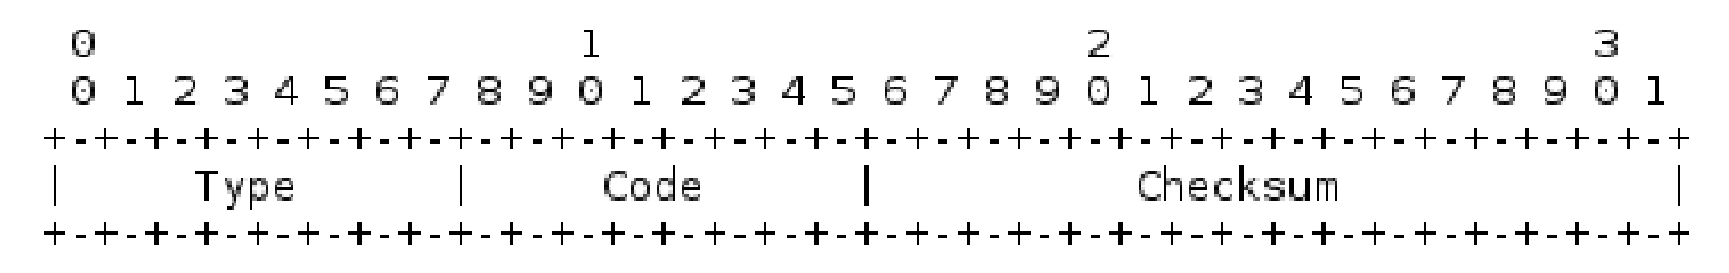
\includegraphics[width=12cm]{./pics/header.eps}
\caption{Champs de l'entête communs à tous les types de message ICMP}
\label{fig:headicmp}
\end{figure}

Le premier champ est celui de type. Il permet, premièrement, de donner le type
du paquet et de l'information à transmettre, et deuxièmement de préciser la
nature des champs qui vont suivre. En effet, comme vu plus haut, les messages
contiennent des champs différents selon le type du message ICMP.  Le deuxième
champ est le code. Il permet de subdiviser le type en donnant des détails plus
précis. Enfin le troisième champ est la somme de contrôle (checksum).
Commençons avec les messages qui possèdent l'ensemble de champs le plus simple.

\begin{figure}[h]
\centering
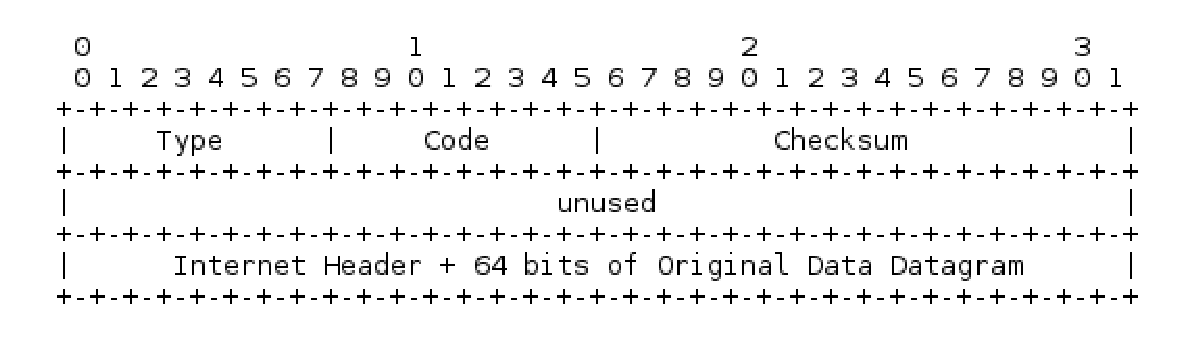
\includegraphics[width=12cm]{./pics/header1.eps}
\caption{Entête des messages de type 3 et 11}
\label{fig:head1icmp}
\end{figure}

Les messages qui utilisent cette organisation sont les messages de type 3 et
11.  Le champ Internet header contient l'entête du paquet qui a provoqué
l'envoie du message ICMP, plus les 64 premiers bits suivant le header. Cela
permet à l'émetteur de retrouver quel paquet à posé problème.

\vspace{1cm}
\textbf{Message de type 3: Unreachable Destination}
Les messages de type 3 sont émis lorsqu'un paquet n'a pas réussi à joindre la
destination (Unreachable destination). Cette erreur peux être dut à plusieurs
facteurs, et les codes permettent de préciser pourquoi le paquet n'a pas pu
rejoindre sa destination.

\paragraph{Code 0: Network Unreachable} Ce code indique que le réseau que
l'hôte essaye d'atteindre n'est pas joignable; ceci étant dut à l'absence de
route vers ce réseau.

\paragraph{Code 1: Host Unreachable} Ce code indique que le réseau à été joint,
mais que le routeur sur ce réseau n'arrive pas à joindre l'hôte à qui délivrer
la trame.

\paragraph{Code 2: Protocole Unreachable} Ce code indique que l'hôte à été
joint, mais que le protocole utilisé n'est pas actif.

\paragraph{Code 3: Port Unreachable} Ce code indique que l'hôte à été joint,
mais que le port utilisé en couche transport n'est pas actif et ne peux donc
être utilisé pour communiquer.

\paragraph{Code 4: Fragmentation needed} Ce code indique que la taille du
paquet dépasse le MTU (Maximum Transmission Unit) et que le flag DF à été mis à
1 dans l'entête IP.  En règle général, si un paquet est plus grand que le MTU,
il doit être fragmenté par le routeur pour être transmis en plusieurs paquets
plus petit. Mais comme le flag DF (Do not Fragment) est mis à 1, le paquet ne
peux être fragmenté. Le routeur émet donc un paquet ICMP de code 4.

Ces codes ont été définis dans la RFC 792, mais depuis d'autre RFC ont ajouté
des codes en plus qui sont utilisés dans des cas plus précis.

\vspace{1cm}
\textbf{Message de type 11: Time Exceeded}
Ce message est envoyé lorsque le TTL d'un paquet à atteint 0. Une autre
utilisation des ces messages est lorsque que le temps de ré-assemblage des
fragments d'un paquet est dépassé. Ces deux cas sont distingué par le code. Ces
messages ont pour destinataire l'hôte qui à envoyé le paquet qui à provoqué
l'erreur.%TODO(vérifier).

\paragraph{Code 0:}
Le code 0 est utilisé pour indiquer que le TTL du paquet posant problème est
arrivé à 0.  Lorsque le TTL d'un paquet arrive à 0, celui-ci est supprimé et un
message ICMP de type 11 et de code 0 est envoyé par le routeur qui à détecté le
problème. Cela permet principalement d'éviter qu'un paquet entre dans une
boucle et qu'il soit relayé à l'infini.

\paragraph{Code 1:} Le code 1 est quant à lui utilisé pour indiquer que l'hôte
n'a pas réussi à réassembler les fragments du paquet IP original dans la limite
de temps prévue à cet effet.


\vspace{1cm}
\textbf{Message de type 5: Redirect Message} Les message de type 5 utilisent
l'entête ci-dessous et servent à faire de la redirection. En effet, lorsqu'un
routeur détecte que le prochain routeur dans lequel va transiter le paquet se
trouve dans le même réseau que l'émetteur de ce paquet, il va envoyer un
message ICMP pour avertir cet hôte (et dans certain cas tous les hôtes sur le
réseau de l'émetteur) qu'il existe un chemin plus court en envoyant directement
les paquets vers le prochain routeur. Ce message ICMP va avoir pour effet de
modifier la table de routage interne à l'émetteur (et dans certain cas tout les
hôtes présent sur le réseau de l'hôte). Concernant le paquet que le premier
routeur à reçu, il va le transmettre vers sa destination.


\begin{figure}[h]
\centering
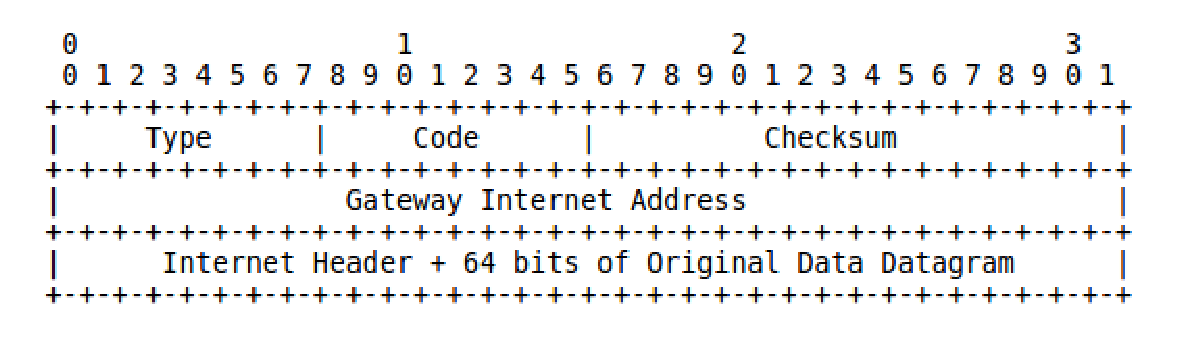
\includegraphics[width=13cm]{./pics/header2.eps}
\caption{Entête des messages de type 5}
\label{fig:head2icmp}
\end{figure}
Le champ Gateway Internet Address contient la l'adresse du routeur auquel il
faut faire transiter le trafique directement pour avoir un chemin de routage
plus court.  Le champ Internet Header contient toujours l'entête du message
ayant provoqué l'envoie du message ICMP plus les 64 bits suivant l'entête. Cela
permet à (aux) hôte(s) de pouvoir modifier leur table de routage en fonction la
destination que cherchait à atteindre le paquet.

\paragraph{Code 0}
Ce code indique que la redirection est adressée à tout les hôtes présent sur le
réseau de l'émetteur du paquet.

\paragraph{Code 1}
Ce code indique que la redirection est adressée à l'émetteur du paquet.

\paragraph{Code 2}
Ce code indique que la redirection est adressée à tout les hôtes présent sur le
réseau de l'émetteur du paquet et aux services.

\paragraph{Code 3} Ce code indique que la redirection est adressée à l'émetteur
du paquet et aux services.

Les messages de code 2 et 3 vont agir sur les services, notamment sur le ToS.

\begin{figure}[h]
\centering
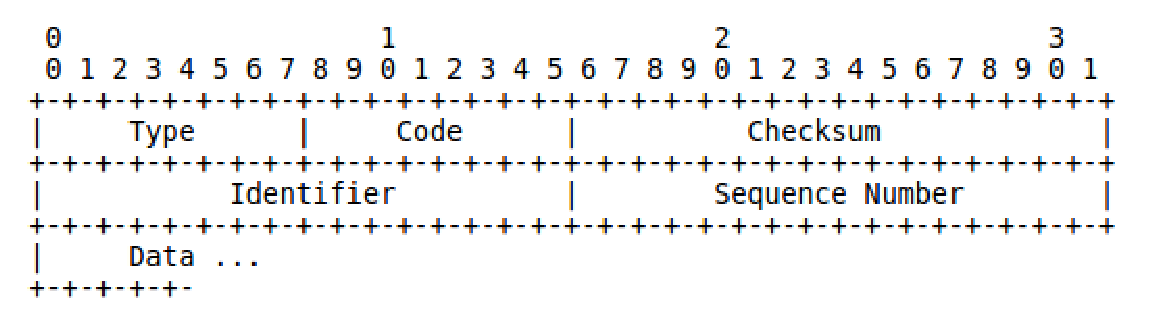
\includegraphics[width=13cm]{./pics/header3.eps}
\caption{Entête des messages de type 0 et 8}
\label{fig:head3icmp}
\end{figure}

\vspace{1cm}
\textbf{Message de type 8 et 0: Echo Request et Reply} Les messages de type 8
et 0 servent à faire des envoies et des renvoies d'information. Ils utilisent
pour cela l'entête ci-dessus. Les messages de type 8 font des envoies
d'informations, appelé echo request. Tandis que les messages de type 0 sont
envoyés en réponse aux echo request et renvoient les informations reçus de
ceux-ci; ils sont appelés echo reply. Etant donnée que les echo reply sont des
réponses aux echo request, l'adresse IP destination des echo reply est
l'adresse IP source des echo request. Ces deux messages peuvent être envoyés et
reçus aussi bien par un hôte que par un routeur. Ce sont notamment les messages
envoyés par la commande {\it ping} qui permettent de vérifier si l'on peux
communiquer avec un hôte ou un routeur.  Les champs Identifier et Sequence
Number aide l'émetteur de l'echo request à associer les echos request qu'il à
envoyés avec les echos reply qu'il à reçus.

\vspace{1cm}
Il y a bien d'autre types et code défini par ICMP, cependant ils sont plus
spécifiques ou devenu obsolètes.


%----------------------------------------------------------------------------------

\subsection{IGMP}
Le protocole IGMP est un autre protocole faisant partit intégrante d'IPv4. Il
permet en effet aux hôtes de communiquer aux routeur mutlicast leur abonnement
à des groupes multicast.  IGMPv2 et IGMPv3 sont les versions les plus utilisées
actuellement. Elles sont respectivement décrient dans le RFC
2236\cite{url-RFC-IGMP2} et RFC 3376\cite{url-RFC-IGMP3}.  Les messages IGMP
sont divisées en trois groupe:
\begin{itemize}
\item Membership Query: Les requêtes d'adhésion: servant aux routeurs pour
faire une demande aux hôtes des groupes auxquels ils sont abonnés.
\item Membership Report: Les rapports d'hôte sur leurs abonnements.
\item Leave Group: Message annonçant l'arrêt d'un abonnement d'un hôte.
\end{itemize}
Tout ces messages sont envoyés avec un TTL de 1, pour éviter que ceci ne
passent d'un réseau à un autre.

\smallbreak
IGMP va donc permettre aux routeurs d'apprendre les groupes d'abonnements des
hôtes qui sont sur le ou les réseaux du routeur. Le routeur dispose d'une liste
des groupes multicast auxquels les hôtes d'un réseau sont connectés, et ceci
pour tout les réseaux auxquels il est connecté.  Pour commencer, le routeur va
envoyer à l'adresse 224.0.0.1, deux (par défaut) Membership Query général à 30
secondes d'intervalles (par défaut).

\smallbreak
Lorsqu'un hôte reçoit un Membership Query, il va initialiser un timer pour
chaque groupe multicast auxquels il appartient. Ces timers sont initialisés
avec un temps aléatoire dont la borne supérieur est spécifié dans le Membership
Query. Ce système de timers permet de ne pas saturer le réseau avec touts les
message IGMP de tout les groupes qui seraient envoyé au même moment.  Lorsque
le timer d'un des abonnements arrive à 0, alors l'hôte émet, en multicast au
groupe en question, un Membership Report.  Si l'hôte reçoit un Membership
Report et que le timer du groupe concerné par le message reçus n'a pas encore
atteint 0, alors l'hôte va arrêter le timer. En effet le routeur sera aux
courant de l'existence du groupe car il aura reçu le même rapport que l'hôte.

\smallbreak
Le protocole IGMP est conçu pour que le routeur sache à quels groupe multicast
sont abonnés les hôte sur les réseaux auxquels il est relié. Cependant le
protocole n'a pas du tout été conçu dans l'optique de fournir la liste des
hôtes avec leurs abonnements.  C'est pour cela qu'une fois que le routeur est
au courant de l'existence d'un groupe, les autre hôtes faisant partie de ce
groupe n'envoie pas de rapport pour ce groupe.

\smallbreak
Lorsque le routeur reçoit un Membership Report il va ajouter le groupe à sa
liste de groupe présent sur le réseau auquel il est connecté. Il va à ce moment
initialiser un timer à 135 secondes (valeur par défaut).  Si il reçoit d'autre
Membership Report pour un groupe existant alors le timer est remis à sa valeur
initiale (de 135 secondes).  Lorsqu'un hôte rejoint un nouveau groupe, il va
émmetre un Unsolicited Membership Report pour s'annoncer dans le groupe, et
ainsi informer le routeur de l'existence de ce groupe ou de la remise à la
valeur initiale du timer.

\smallbreak
Le dernier cas de figure est lorsqu' un hôte veut se désabonner d'un groupe: il
va donc arrêter de traiter les messages à destination du groupe multicast. Si
l'hôte est le dernier de son groupe alors il va envoyer un Leave Group à
l'adresse 224.0.0.2.  Si il n'est pas le dernier, il peux simplement ne rien
faire et se désabonner du groupe, il ne sera plus concerné par les messages à
destination du groupe. Etant donné qu'il y a d'autres membres dans le groupe
ceci s'occuperont de "maintenir le groupe en vie".  En revanche si l'hôte ne
sais pas si il est le dernier hôte dans le groupe rien ne l'empêche d'envoyer
un Leave Group.

Lorsque le routeur reçoit un Leave Group, il sais qu'un membre à quitté le
groupe. Ce qui l'intéresse est de savoir si il y a encore des membres dans le
groupe en question ou si s'est le dernier membre qui vient de quitter le
groupe. Il va pour cela envoyer deux Membership Query spécifiquement au groupe
en question. Si aucune réponse n'est reçut le groupe est considéré comme
n'ayant plus de membre et il est oublier du routeur.  Si jamais les hôte
n'annonçait pas leur retrait du groupe (comme cela à été évoqué plus haut) et
qu'il n'y avait plus d'hôte faisant partit du groupe, alors le groupe serait
considéré sans membre et oublié lorsque le timer du routeur arriverait à 0 pour
le groupe en question.

\smallbreak
Le dernier point pour que tout cela fonctionnent, est qu'il faut que le routeur
envoie régulièrement des Membership Query général pour qu'il maintiennent à
jour sa table des groupe présent sur le réseau, sinon ceux-ci serait oublier
une fois le timer arrivé à expiration.

%----------------------------------------------------------------------------------------


\subsection{DHCP}
Le protocole DHCP (Dynamic Host Configuration Protocol) sert à l'auto-configuration
des interfaces. Plus précisément, il  permet d'attribuer une adresse IP à une
interface et de lui faire parvenir d'autres information essentielle pour le
fonctionnement de l'interface sur le réseau. La version initiale de DHCP fut décrite
dans le RFC 1531\cite{url-RFC-DHCP1}, mais cette version fut rendue obsolète par un autre
RFC, lui même rendue obsolète par le RFC 2131\cite{url-RFC-DHCP2} qui est la dernière version non
obsolète. Voyons comment une interface peut ce configurer auprès d'un serveur DHCP.

\begin{figure}[h]
\centering
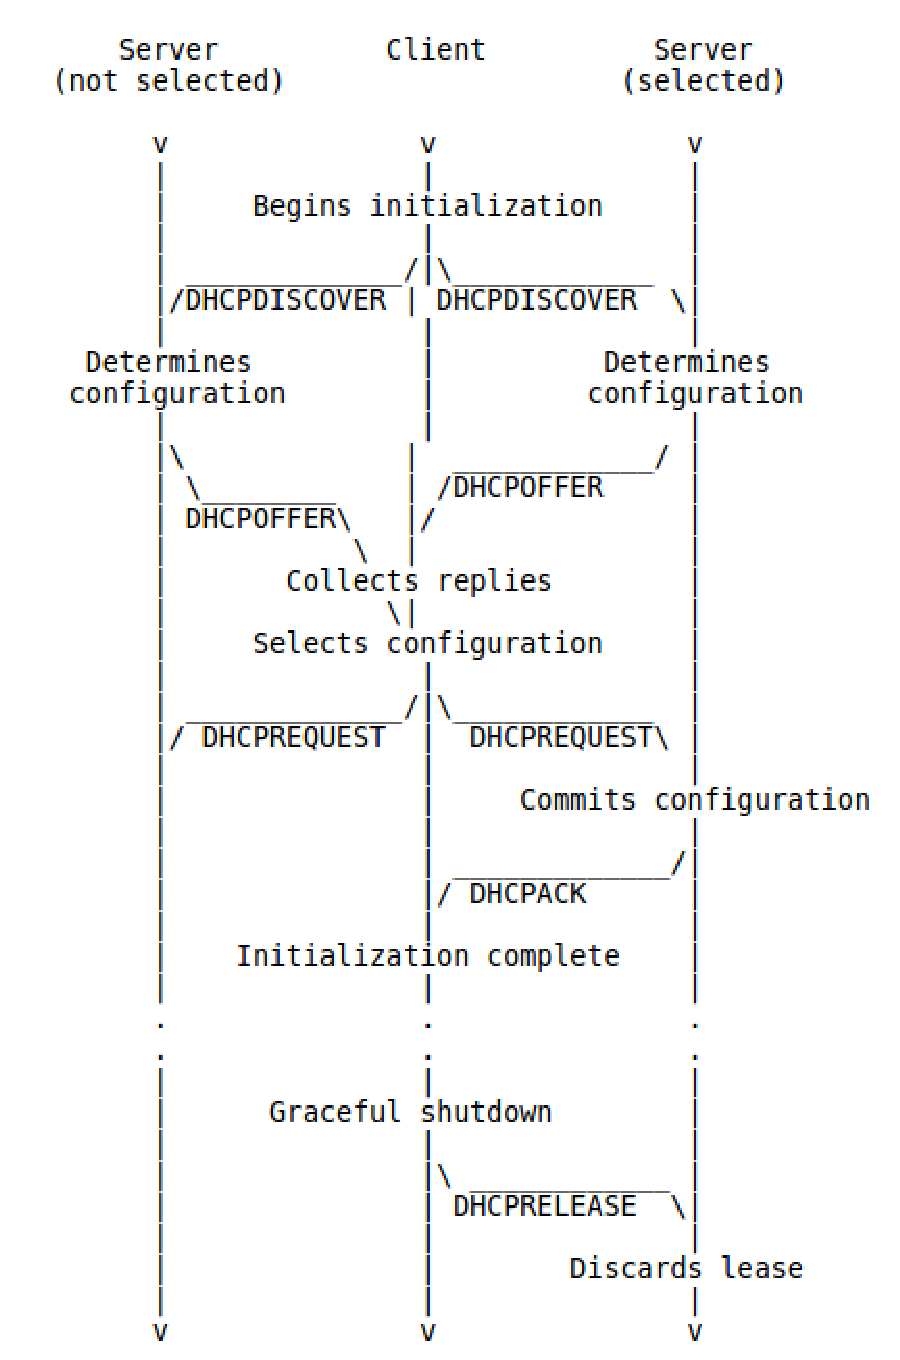
\includegraphics[width=6cm]{./pics/timeline_dhcp.eps}
\caption{Déroulement de la négociation DHCP}
\label{fig:timelinedhcp}
\end{figure}

Lorsqu'une interface, qui n'a pas d'adresse IP, souhaite en recevoir une, elle
va émettre un message DHCPDISCOVERY en broadcast sur son réseau. Des agents DHCP
peuvent faire passer
ce message DHCP sur un autre réseau si le serveur DHCP (qui distribue les
adresses) ne se trouve pas sur le même réseau que l'hôte qui fait la demande.
L'hôte va utiliser comme adresse IP 0.0.0.0.

\smallbreak
Etant donné que le message est envoyé en broadcast, tout les hôtes sur le
réseau vont recevoir le message, et en particulier le ou les serveurs DHCP qui
pourraient s'y trouver. Si cela est le cas, ceux-ci vont répondre avec un
DHCPOFFER. Ce message contient entre autre l'adresse IP proposé pour le client
souhaitant se configurer, ainsi que le masque du réseau. A ce
moment là l'adresse n'est pas encore attribuée et réservée pour l'hôte étant
donnée qu'il peut refuser l'offre et accepter l'offre d'un autre serveur. Si
jamais l'hôte ne reçoit aucun DHCPOFFER, il va ré-émettre un DHCPDISCOVERY. Si
il reçoit un ou plusieurs DHCPOFFER, l'hôte va devoir choisir une configuration
parmis celles qui lui sont proposées. Une fois ce choix fait, il va informer les serveurs DHCP de
son choix à l'aide d'un message DHCPREQUEST émis en broadcast. Ce message va
contenir l'identifiant du serveur DHCP retenu ainsi que la configuration
souhaité par l'hôte (adresse IP et masque du réseau). Ce message peut être
interprété de deux manières différentes selon le serveur:
\begin{itemize}
\item Si ce n'est pas le serveur retenu, il considère le message comme une
déclinaison de l'offre.

\item Si c'est le serveur retenu, il va sortir l'adresse attribuée à l'hôte de la
plage d'adresse libre pour ne plus l'attribuer à un autre hôte. Il va ensuite
émmettre un message DHCPACK contenant la configuration effective de l'hôte avec
notamment: l'adresse IP, le masque du réseau, la durée du bail, l'adresse
de la passerelle par défaut et l'adresse du serveur DNS.  Si pour quelque
raisons que ce soit le serveur n'est pas capable d'attribuer l'adresse proposée dans l'offre
(par exemple si l'adresse à été attribuée entre temps), le serveur émet un
DHCPNAK pour avertir l'hôte que l'adresse n'est plus disponible. L'hôte devra
alors recommencer la procédure pour obtenir une configuration.
\end{itemize}

\smallbreak
Enfin si le serveur ne reçoit pas de message DHCPREQUEST, la procédure
s'arrêtera à ce moment et l'adresse n'étant pas encore attribuée à l'hôte elle
reste disponible pour être attribuée à d'autre hôte. 

\smallbreak
Arrive la dernière étape.
Si l'hôte reçois un message DHCPACK, il peux prendre en compte la
configuration (adresse IP, masque du réseau, DNS, passerelle par défaut et
durée de bail). Il va effectuer une dernière vérification pour s'assurer que
l'adresse qui lui à été attribué est bien unique sur le réseau pour éviter
d'avoir deux hôte avec la même adresse. Il va pour cela utilisé le protocole
ARP et la méthode de vérification vu plus haut. Si jamais l'adresse est déjà
utilisé par un autre hôte, il va envoyer un message DHCPDECLINE au serveur DHCP
pour lui indiquer qu'il n'utilisera pas la configuration proposée par celui-ci,
et il va recommencer la procédure pour pouvoir obtenir une nouvelle
configuration.

\smallbreak
Si jamais l'adresse proposé par le serveur est unique sur le réseau, la
configuration est terminé et l'hôte peut utiliser l'adresse (durant la durée du
bail de celle-ci).  Dernier cas possible, si jamais le l'hôte ne reçoit pas de
DHCPACK ou de DHCPNAK, il va réémettre le message DHCPREQUEST pour espérer
recevoir une réponse du serveur.

\smallbreak
Tout au fil des différents messages échangés, le client est identifié grâce au
champ client identifier, et le serveur grâce au champ server identifier.

L'hôte est donc configuré et peut utiliser son adresse. Cependant, il ne peut
l'utiliser que durant la durée de son bail. Une fois le bail expiré, l'hôte ne
peux plus utiliser son adresse. Lorsque l'hôte a reçu le message DHCPACK du
serveur, celui-ci lui a transmis la durée du bail. De cette durée, l'hôte va
en extraire deux temps noté T1 et T2. T1 correspond à la moitié de la durée du
bail et T2 à 0.875 fois la durée du bail. Ces temps sont exprimés de manière relatif
étant donnée que les horloges du serveur et de l'hôte ne sont pas
synchronisées.  Une fois que l'hôte à atteint le temps T1, il va chercher à
contacter le serveur qui lui à attribué sa configuration avec un message
DHCPREQUEST pour étendre la durée de son bail. Ce message est émis de manière
unicast. A ce moment l'hôte est entré en état RENEWING. Si l'hôte reçoit un
message DHCPACK du serveur lui accordant un prolongement de la durée de son
bail, alors il va sommer le temps qu'il avait insérer dans le DHCPREQUEST avec
la durée accordée par le serveur et qui se trouve dans le message DHCPACK.
L'hôte retourne dans l'état BOUND. Cependant l'hôte n'est pas obligé d'attendre
T1 pour pouvoir étendre son bail.  Si jamais l'hôte ne reçoit pas de réponse
DHCPACK avant l'arrivé de T2, il passe en état REBINDING. A ce moment il va
émettre un DHCPREQUEST en broadcast pour espérer pouvoir étendre son bail
auprès de n'importe quel serveur DHCP. Pour parer aux éventuels cas de perte de
DHCPREQUEST, l'hôte va renvoyer un message une fois la moitié de la durée entre
T1 et T2 passé, en état RENEWING; et une fois la moitié de la durée entre T2 et
la fin du baille , en état REBINDING (et avec un minimum de temps de 60
secondes).  Si malgré tout, la durée du bail venait à expirer, alors l'hôte ne
posséderait plus de configuration réseau et ne pourrait plus communiquer avec
d'autre hôtes. Il rentre alors en état INIT; il doit alors recommencer la
procédure pour obtenir une configuration.

\smallbreak
Cependant,dans ce cas comme dans d'autre, l'hôte peut ré-utiliser une
configuration précédemment utilisée. Cela permet de raccourcir la négociation
entre l'hôte et le serveur DHCP. L'hôte va directement commencer la négociation
en faisant un DHCPREQUEST en broadcast et contenant la configuration qu'il
souhaite ré-utiliser. Le serveur concerné par l'attribution antérieur de la
configuration va donc accepter la demande de l'hôte à l'aide d'un DHCPACK ou la
refuser, si la demande n'est pas correct ou si l'adresse est utilisé par un
autre hôte, à l'aide d'un DHCPNAK.  Cette négociation se fait de manière
similaire à une négociation complète, elle a juste été raccourci en enlevant
quelques étapes non indispensables.

\begin{figure}[h]
\centering
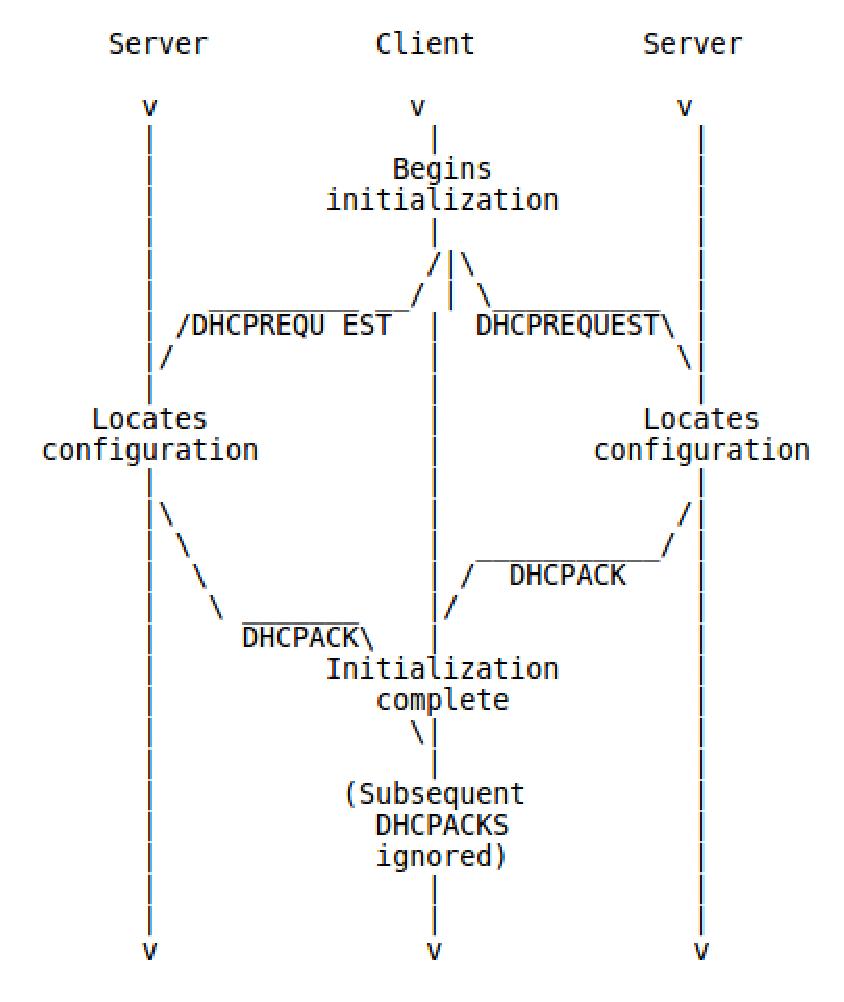
\includegraphics[width=6cm]{./pics/timeline_dhcp_reuse_add.eps}
\caption{Déroulement de la négociation DHCP pour la réutilisation d'une configuration}
\label{fig:timelinedhcpreuseadd}
\end{figure}

%---------------------------------------------------------------------------------

\subsection{PMTU discovery}
Le protocole PMTU discovery (Path MTU discovery) décrit dans le RFC
1191\cite{url-RFC-PMTU}, permet de trouver le plus petit MTU d'un chemin entre
l'émetteur et le récepteur. Cela permet d'éviter la fragmentation des paquets
IP ce qui permet entre autre de soulager la charge des routeurs.  L'hôte
souhaitant connaître le plus petit MTU pour un chemin vers autre hôte va
envoyer un paquet avec un certain MTU et en plaçant le bit DF de l'entête sur 1
pour éviter la fragmentation du paquet. Ainsi si le MTU est trop grand à un
moment donné du chemin, le routeur ne pourra pas fragmenter le paquet mais ne
pourra non plus pas transmettre le paquet en l'état. Il va alors détruire le
paquet, et émettre un message ICMP de type 3 et de code 4 vers la source du
paquet, signalant que la destination n'est pas joignable, et que cela est dut à
un paquet nécessitant une fragmentation or celle-ci est interdite. Le MTU est
donc trop élevé. Le message ICMP contient le MTU qu'il faut passé le routeur.
L'émetteur va alors créer un nouveau paquet avec le nouveau MTU. Il fera cela
autant de fois que cela est nécessaire pour déterminer le MTU du chemin.

\subsection{DNS}
Le protocole DNS (Domain Name System) permet de faire de la résolution
d'adresse.  Cela est permis grâce à des échanges avec un ou plusieurs serveur DNS.
Un serveur DNS va faire de la traduction de nom de domaine, notamment en adresse IP. Pour
simplifier, le nom de domaine, facilement retenu par un être humain va être
traduit en adresse IP pour être utilisée par l'ordinateur.  Nous n'aborderons
pas plus le fonctionnement de DNS car s'est un protocole de couche application
et qu'il n'est pas essentiel au fonctionnement d'IPv4. Cependant il reste
essentiel dans l'utilisation d'Internet, aujourd'hui, par des êtres humains.


\section{Passage de IPv4 à IPv6}
\subsection{Raison du passage de IPv4 à IPv6}
\subsubsection{Problème posé par IPv4}
//Pénrurie, adressage privé/publique compliqué
% Il se trouve que apparement il y a des problemes de
% penurie d'adresses meme dans certaines reseau prive`
% http://blog.erratasec.com/2013/12/dod-address-space-its-not-conspiracy.html#.WAf_d7Wf21F

PROBLÈMES DE IPV4

ÉPUISEMENT DES ADRESSES
Lorsque IPV4 a été développé dans les années 70-début des années 80, personnes n'aurait imaginé qu'il y aurait un jour autant d'interfaces qui se connectent à Internet. On pensait qu'une adresse sur 32 bits serait suffisante. De plus, les plages d'adresses étaient distribuées généreusement au début. Cela veut dire que l'on attribuait des adresses permettant un nombre d'interfaces beaucoup plus grand que nécessaire.
Cependant, avec la croissance du nombre d'utilisateurs, la plage d'adresses IPV4 disponible a diminué progressivement. C'est en février 2011 que la réserve de bloc libres d'adresses publics IPV4 de l'IANA (Internet Assigned Numbers Authority) est arrivée à épuisement.
Afin de résoudre ce problème, plusieurs techniques ont été proposées.
La première a été le changement de teechnique d'adressage. On est passé de la technique de classe d'adressage IP à la technique Classless Inter-Domain Routing. Ceci à permis une meilleure efficacité dans la distribution des adresses IP grâce à la création de réseau de tailles intermédiaire. En effet, avant on ne disposait que de réseau de 3 tailles différentes.
Les politiques d'assignement d'adresses ont également été rendu plus stricte afin de mieux tenir compte des besoin réels des demandeurs d'adresses IP.
Il a aussi été décidé d'utiliser des blocs autrefois réservé comme 14.0.0.0.
Sur base de volontarisme, des blocs autrefois attribués généreusement ou alors des IP non utilisées ont été récupérées. 
Finalement, il a été remarqué qu'il n'était pas nécessaire que chaque interface a son adresse IP public et le protocole NAT a été développé afin de regrouper plusieurs interface sous une même adresse IP. Ce protocole est de plus en plus utilisé dans IPV4 depuis la fin des années 90.

Fonctionnement du NAT dynamique (Network Adress Translation)
Le NAT est une technique utilisée au niveau du routeur. Le principe du NAT est
que le routeur fait correspondre à une adresse IP une autre adresse IP. En
général cette technique est utilisée pour avoir une même adresse IP pour tout
un réseau comme un intranet ou encore un réseau domestique. Dans ce réseau,
toutes les interfaces - même le routeur - auront une adresse privée. Le routeur
dispose en plus de cela de une ou plusieurs adresses publics avec lesquelles il
est connecté à internet. Une adresse privée est une adresse qui est utilisée à
l'intérieur d'un réseau local. Les adresses privées peuvent être choisies parmi
les suivantes: 10.0.0.0/8, 172.16.0.0/12 ou 192.168.0.0/16.  Lorsqu'une
interface envoie un paquet vers l'extérieur du réseau, le routeur effectue
plusieurs changements. Il traduit d'abord l'adresse privée en adresse public et
la met dans l'en-tête du paquet. Puis il change tous les checksums qui tiennent
compte de l'adresse IP. Enfin, il garde en mémoire dans une table la
correspondance entre adresse privée/adresse public comme ci-dessous.  <tableau
adresse public / privée >
Cela n'est cependant pas suffisant. En effet, lorsqu'un paquet arrivera de l'extérieur du réseau,  et si tous les interfaces utilisent la même adresse public sans distinction supplémentaire, le routeur ne saura pas à quelle interface envoyer le paquet. 
Une solution à ce problème existe pour les protocoles utilisant les ports comme TCP et UDP. Le routeur ajoute une information supplémentaire dans la table qui est le port source d'où vient le paquet. Les ports, qui sont implémentés dans la couche transport (couche 4), sont des sortes de ''portes'' qui permettent de communiquer avec un système d'exploitation. Le numéro de port est un numéro choisit aléatoirement entre 1024 et 65535.
Pour illustrer le fonctionnement du NAT imaginons qu'une interface A dont l'ip est 192.168.0.1 veut envoyer un paquet à l'interface B d'ip 217.70.184.38. Le port source est le port 10277 et le port destination est le port 80. 
La table NAT ressemblera à ceci:

<TABLE NAT complète > 

La box internet enverra le paquet:

L'interface B répondra en envoyant le paquet:

Lorsque la box reçoit ce paquet, elle voit que le port de destination est le port 10277. Elle cherche ensuite le port correspondant dans sa table NAT. Lorsqu'elle le trouve elle effectue les changements nécessaire sur le paquet et transmet le paquet à l'interface A.
Mais même si cette solution fonctionne la plupart du temps, la probabilité est faible que 2 interfaces envoient des paquet sur les même port. C'est pour éviter cela que la box change le port source lorsqu'elle reçoit un paquet de l'interface A. Ainsi on s'assure que aucun port n'est utilisé plusieurs fois. Enfin, pour éviter de saturer les ports utilisés, un compteur est associé à chaque paire adresse public/adresse privée. Lorsqu'il n'y a pas de trafic entre une adresse privée et l'extérieur durant une durée fixée, le port qui lui est associée peut être réutilisé pour une autre adresse privée.

Le NAT dynamique apporte cependant un grand problème. Lorsqu'une interface
extérieur veut se connecter à une interface dans le réseau, elle ne dispose
d'aucune autre information que l'adresse IP public. Si elle envoie alors un
paquet à cette adresse, le routeur qui le réceptionnera ne saura pas quoi faire
avec et le paquet sera perdu.  On a réussi à pallier à ce problème grâce au
port forwarding. 

PORT FORWARDING

NAT STATIQUE


\subsubsection{Solutions}
//NAT,IPv6
\subsection{Différence entre IPv4 et IPv6}

% MOSSI

Il est important de comprendre que l'IPv6 est beaucoup plus qu'une extension de
l'adressage IPv4. IPv6, d'abord défini dans la RFC 2460, est une mise en oeuvre
complète de la couche réseau de la pile TCP/IP et il couvre beaucoup plus que
l'extension de l'espace d'adressage simple à partir de 32 à 128 bits (le
mécanisme qui augmente la capacité d'IPv6 à allouer presque un nombre illimitée
d'adresses à tous les appareils dans le monde pour les années à venir).IPv6
offre de nombreuses améliorations par rapport à IPv4, et le tableau ci-dessous
compare le fonctionnement de IPv4 et de IPv6.

Systéme de routage beaucoup plus efficace. Les paquets IPv6 ne sont plus
fragmenté par les routeurs.
	
La qualité de service(QoS) intégrée. Alors que IPv4 n'a aucun moyen de
distinguer les paquets sensibles au retard de transferts de données en vrac, ce
qui nécessite de nombreuses solutions de contournement, mais IPv6 le fait.
	
L'élimination du NAT pour élargir les espaces d'adressage. IPv6 augmente la
taille de l'adresse IPv4 de 32 bits (environ 4 milliards) à 128 bits
(suffisamment pour chaque molécule dans le système solaire).
	
La sécurité de la couche réseau intégré (IPsec). La sécurité a toujours été
un défi en IPv4, mais elle est une partie intégrante de l'IPv6.
	
L'autoconfiguration d'adresse pour l'administration réseau plus facile. De
nombreux installations IPv4 ont été compliquées par le routeur par défaut
manuelle et l'attribution d'adresse. IPv6 gère cela de manière automatisée.
	
L'amélioration de la structure d'en-tête permet d'alléger le traitement. La
plupart des champs dans l'en-tête IPv4 étaient facultatifs et utilisés
fréquemment. IPv6 élimine ces champs (les options sont traitées différemment).





\section{Conclusion}
\label{sec:ccl}

\addcontentsline{toc}{section}{Références}
\bibliographystyle{plain}
\bibliography{rapport}

\end{document}
